%\documentclass[10pt,journal,twoside]{IEEEtran} % for editor use only for final preprint

% For initial draft
\documentclass[10pt,draftcls,journal,onecolumn]{IEEEtran}
\usepackage{endfloat}
%\usepackage[switch]{lineno}
\usepackage{lineno}


\usepackage{cite}
\usepackage{amsmath,amssymb,amsfonts}
\usepackage{graphicx}
\usepackage{siunitx}
\usepackage[colorlinks=true,allcolors=blue]{hyperref}
\usepackage{cleveref}
\crefname{equation}{}{}
\Crefname{equation}{}{}
\crefname{figure}{Fig.}{Figs.}
\Crefname{figure}{Fig.}{Figs.}
\crefname{table}{Table}{Tables}
\Crefname{table}{Table}{Tables}
\usepackage{booktabs}
\usepackage{multirow}


\title{Braves Pink Sea Perch Technical Report} % Your title goes here
\author{Kaitlin Coulanges, Julia Khabinskiy\thanks{Author for correspondence: 427jkhabinskiy@frhsd.com},Sejal Nagrani, Paula Reynaga, Renee Robinson and Ashriel Vellore\thanks{Authors are with the Science \& Engineering Magnet Program, Manalapan High School, 20 Church Lane, Englishtown, NJ 07726, USA}} % Authors names here
% First author is normally a special position
% Corresponding author is a special position
% Last author normally most senior
% You can put your names in any order you decide but be aware of these conventions
\date{\today}
\markboth{Journal of Science \& Engineering, Vol.~1, No.~2,~December 13, 2024}{Lennon \MakeLowercase{\textit{et al.}}: She loves you} % may need shortened form of author names or title
\setcounter{page}{1} % LEAVE FOR EDITOR
\newcommand{\keywords}{submersible, remotely operated vehicle, submarine, naval architecture, Sea Perch} % put your keywords here, lower case unless proper noun or acronym, separated by commas
\makeatletter
\AtBeginDocument{
\hypersetup{%
pdftitle={\@title},
pdfauthor={\@author},
pdfsubject={physics},
pdfkeywords={\keywords}}}
\IEEEoverridecommandlockouts
\IEEEpubid{\makebox[\columnwidth]{10.64804/xxxxxxxx~\copyright~2026 J S\&E \hfill} \hspace{\columnsep}\makebox[\columnwidth]{ }}% LEAVE FOR EDITOR
\makeatother







\begin{document}
\linenumbers % for editor use
\maketitle

% AUTHORS PUT YOUR ABSTRACT HERE
\begin{abstract}
This Technical Design Report details the iterative design process utilized in creating the Manalapan Braves Pink’s ROV, BARBIE. As a rookie team, we researched the various components that are needed to ensure a successful marine ROV. Our team proposed multiple design iterations, including the use of a claw, hooks, and 3d printed hands.

After rigorous exploration and discussion, our team settled on a design using a curved framework as well as one 3D-printed hook to balance out the weight of the curved design. We decided on a small ROV, to increase agility in the water. After finalizing the placements and arrangements of all pieces in our CAD model, and gaining all the necessary resources, we began construction of the robot. We also wanted to add a camera to our design, so we could have clear vision underwater to better maneuver the ROV. We found over 4 cameras across various sources that were both cost-effective and viable to our design. Ultimately, we decided on the LCD fishing camera with night vision.

Our 3D printed hook, after refining its dimensions and arrangement, effectively completes the given task as well as provides stability to the ROV by counteracting the weight of the framework of the ROV. We wanted to implement various other electronics into our design to improve performance, but this was challenging under the \$25 limit in our class. As we become more experienced, we hope to compete in the open class, so that we can afford more materials and make a more sophisticated robot.
\end{abstract}

\begin{IEEEkeywords}
\keywords
\end{IEEEkeywords}

\section{Introduction}
%\IEEEPARstart{T}{he electric} potential $V$ of a particle 
% The editor will do this
The introduction should work from broad to specific. Give major important background information or set up the major concepts to be used or tested. Set up the key research questions or hypotheses to tested. Optionally, give top level overview of method to be used. 

This section also acts as a literature review of other important work in the field and relevant to the questions at hand. An example of how to cite something is here \cite{tipler}. Here is another example \cite{openstax}. The actual citation data is provided in the file \texttt{example.bib} which you should also look at. Two more examples are \cite{rombauer:1931:joy, binzel:1988:hemispherical}. Please do not type in your references to try to force them to be MLA or whatever format as these are not the right formats for an IEEE paper; \LaTeX\ and \texttt{bibtex} know how to do the necesary formatting. Typing in your references in some other format will make more work for the editors and they will be grumpy. If you absolutely cannot figure out how to do references, pick a consistent label name for each reference to use, and the editor may help you out. 

Equations are appropriate here if needed; symbols should be consistent throughout the paper. An example equation is:
\begin{equation}
\sum \vec{F} = m \vec{a}.
\label{eq:fma} % example label for use with cleveref
\end{equation}
Equations receive punctuation; a period at the end is appropriate if it is the end of a sentence, or a comma if there is more to follow such as explanation of the symbols. Two ways to explain the symbols used are a list of symbols, or to explain them in the text. For the preceeding example in \cref{eq:fma}, $m$ is the mass in \unit{\kilo\gram}, while $\vec{a}$ is the acceleration in \unit{\meter\per\second}. J S\&E uses the \LaTeX\ \texttt{siunitx} package to format units consistently. Please do not type in your units manually, use the macros. Typing in your units manually will make more work for the editors and they will be grumpy. If you absolutely cannot figure out units or equations, write something simple with no formatting (F=ma here) and the editor may help you out. 

Remember in science we do not ``prove'' hypotheses, we can disprove alternatives by falsifying them, and that any hypotheses we propose must be testable (as in there must be a way to show it was wrong). At the end of the introduction you normally introduce the research question your are out to answer and set up the testable hypotheses you will test in this article. 

For initial submission it is common to set the paper to print doublespaced and with line numbers. Do not remove these it makes it easier for reviewers to comment. After initial review, the editor may switch it over to look like a preprint to aid in final formatting. Do not do this yourself! 






\section{Methods and Materials}
Provide all methods and materials in a form that is replicable by a competent scientist or engineer. This section is normally written in past tense, e.g. ``We used an Easy Bake Oven (Hasbro; Pawtucket, RI) to evaporate plutonium samples to complete dryness...'' Key pieces of equipment or key reagents and materials should be listed with a source where they were obtained from. 

\textbf{Do not include results in your methods.} The methods tell other scientists how to replicate what you did. \textbf{Do not provide a laundry list or recipe of steps like you copied from a lab handout or an AI; these will be rejected.} 

It is appropriate to put links to code or datasets; put long items in an appendix or provide online.  For example, all code used to generate this example is provided at \url{https://github.com/devangel77b/jse-electricity-template/}. 


\subsection{Use of subsections}
Consider breaking the methods into subsections, either for different major methods or parts of the experiment. Alternatively you could break it down into subsections based on things like: experimental subjects; drop testing; statistical analyses, etc. Major models or equations are appropriate here if they explain how you are handling your data. 






\section{Results}
The results should deal with ``just the facts'' exactly what you saw or measured, without interpretation. You should include graphs, tables, summary statistics, and results of statistical tests here. The key thing here is that you are reporting truthfully what you saw as just the facts; people may differ on the interpretations but results ought to be taken at face value unless your methods are flawed. Figures and tables must be numbered and must be referred to in the text. 

An example of a figure is \cref{fig:foo}. Note that the figure reference name must begin with \texttt{fig:} in order for the \LaTeX cleveref macros to properly parse it. 
\begin{figure}
\begin{center}
%Image file would go here 
% \includegraphics{figures/fig1.png}
\includegraphics{figures/newfig1.pdf}
% \includesvg{figures/fig2.svg}
\end{center}
\caption{This is a caption. Captions for figures go below the figure. For IEEE format the width is 3.5 inches, or 7.16 inches for two columns.}
\label{fig:foo}
\end{figure}
    
An example of a table is \cref{tab:bar}. 
\begin{table}
\caption{This is a table. Captions for tables go above the table.}
\label{tab:bar}
\begin{center}
\begin{tabular}{cc}
\toprule
$x$ & $\bar{x}$ \\
\midrule
0 & 1 \\ 
1 & 0 \\
\bottomrule 
\end{tabular}
\end{center}
\end{table}








\section{Discussion}
The discussion is where you interpret the meaning of your results and whether they support your hypotheses or refute alternative hypotheses. You should refer to tables, figures, etc by number and use them in supporting your arguments here. To refer to a figure do like this: \cref{fig:foo} shows the third Zonklar moment as a function of $t$. To refer to a table like \cref{tab:bar}, do like this. 











%\section*{Contributions}
\section{Acknowledgement}
Keep it short or the editors will shorten it for you. JL wrote and PM wrote the lyrics. GH contributed rhythm guitar tracks. RS contributed drumbeats. Do not write long essays about Ms Komitas, Dr E, or the S\&E program here; we don't need or want fluff. 







%\end{thebibliography}
\bibliographystyle{IEEEtran}
\bibliography{example.bib}

% Images for the biography should be a 1in wide by 1.25 high or a 5:4 aspect ratio
% Keep your biography short and to the point or the editors will shorten it
\begin{IEEEbiography}[{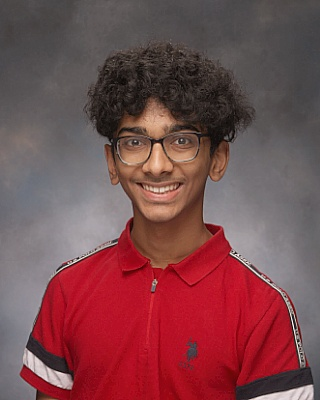
\includegraphics[width=1in,height=1.25in,clip,keepaspectratio]{sayyagari.jpeg}}]{Saketh Ayyagari} is a senior in the Science and Engineering Magnet Program at Manalapan High School. He is also an intern at Commvault in Tinton Falls, NJ, founder of the Cyber Security Club, member of the Cyber Security Team, and captain of the FIRST Technology Challenge robotics team \#13115 Brave Robotics. 
\end{IEEEbiography}

\begin{IEEEbiography}[{\includegraphics[width=1in,height=1.25in,clip,keepaspectratio]{vcollemi.jpeg}}]{Victoria Collemi} is a senior in the Science and Engineering Magnet Program at Manalapan High School. She is also an intern at Girl in Space Club, president of the Robotics Club, and founder and president of the Rocketry Club. 
\end{IEEEbiography}
\vfill
\newpage 
\begin{IEEEbiography}[{\includegraphics[width=1in,height=1.25in,clip,keepaspectratio]{kshah.jpeg}}]{Krish Shah} is a senior in the Science and Engineering Magnet Program at Manalapan High School. He is also an intern at Commvault in Tinton Falls, NJ, and is a member of the FIRST Technology Challenge robotics team \#13115 Brave Robotics. 
\end{IEEEbiography}

\begin{IEEEbiography}[{\includegraphics[width=1in,height=1.25in,clip,keepaspectratio]{ktomazic.jpeg}}]{Kevin Tomazic} is a senior in the Science and Engineering Magnet Program at Manalapan High School. His current senior project is to create a robot designed to autonomous clean beaches. He is also the only department head of the Manalapan High School Drama Club tech department. 
\end{IEEEbiography}
\vfill
\end{document}

